% Copyright (C) 2010 Thomas L. Kula
% All Rights Reserved
%
% See the file LICENSE for license terms.
\documentclass[12pt]{article}
\usepackage{graphicx}
\usepackage{rotating}
\usepackage{fix-cm}
\usepackage{multirow}
\setlength{\paperwidth}{5.5in}
\setlength{\paperheight}{8.5in}
\setlength{\textheight}{7.45in}
\setlength{\topmargin}{-1.0in}
\setlength{\oddsidemargin}{-0.5in}
\setlength{\evensidemargin}{-0.5in}
\setlength{\textwidth}{4.0in}
\setlength{\parindent}{0in}
\setlength{\parskip}{3mm}
\usepackage[print]{booklet} \nofiles
\source{\magstep0}{5.5in}{8.5in}
\target{\magstep0}{11in}{8.5in}
\setpdftargetpages
\pagestyle{empty}
\begin{document}


\begin{center}
{\fontsize{36}{48}\selectfont \textsc{Haiku a Day }}
\end{center}

\vspace*{3.5cm}

{\fontsize{20}{40}\selectfont 

Dawn jerked earlier

By those who muddle with time

Twice-yearly rage wells

}

\vspace*{5.0cm}
\begin{center}
{\large{Issue 64: October 2010}} \\[5mm]
{\fontsize{8}{8}\selectfont  \textsc{ St. Joshua Norton Press }} \\[1mm]
{\fontsize{6}{6}\selectfont Mathom House in Midtown \textbar The People's Republic of Ames }
\end{center}


\newpage

When I become Dictator of Something, the first thing against the
wall is Daylight Savings Time.

--- Thomas

http://kula.tproa.net/had/ \\
kula@tproa.net

Download this and previous HADs at the website, so you can
print out your own (DIY, yeah!) or if you want me to send
you one, send me your address, and maybe a stamp if you
are feeling nice. Or send me something you've made ---
trades always appreciated, postcards are nice too.

\vspace*{2.5cm}

1 October 2010

A hiss, imperfect \\
Cups inside of it perfection \\
Classical records

2 October 2010

Rust red staining ground \\
Where a metal pylon strains \\
Holding back the sky

3 October 2010

What beaten springs up \\
Stronger than just laying there? \\
Egg whites become foam

\newpage

4 October 2010

A glass jar holding \\
Tasty fermented delight \\
Kimchi, I salute!

5 October 2010

Round becomes angles \\
Smooth fractures, jagged edges \\
Once high breaks down low

6 October 2010

On the nightstand tall \\
Casting beams into the night \\
Lamp, keep shining on

7 October 2010

With a rental car \\
I feel the urge to pack like \\
I am invading

8 October 2010

Pounds of Chinese food \\
More than any one can eat \\
Neat rows in the fridge

9 October 2010

The store of Norsemen \\
Providing weird glowy things \\
The perfect present

10 October 2010

On the stage lights dim \\
In the spotlight two people \\
Say important things


\newpage

11 October 2010

Fancy rental car \\
Makes me feel like an asshole \\
And gets bad milage

12 October 2010

Just a few days gone \\
Yet discombobulation \\
Rears its fuzzy head

13 October 2010

The brain, warmed by thought \\
The buzz of research humming
Spent, grinds to a halt 

14 October 2010

What a vast network \\
Subterranean, gurgling \\
Just to get water

15 October 2010

After a long wait \\
I'm staying where I'm at now \\
Instead of Pittsburgh

16 October 2010

Once state of the art \\
This tiny box obsolete \\
TI-85

17 October 2010

Where did you come from? \\
Little tack sits on the floor \\
Causes big ruckus


\newpage

18 October 2010

Focus emerges \\
Productive, but a down side \\
A back full of knots

19 October 2010

My old nemsis \\
Alarm clock, never happy \\
Strident tones rebuke

20 October 2010

Dusty smokey crunch \\
Rustling in the wind, stops \\
Wet earthy blanket

21 October 2010

Unflinching, the Moon \\
Outshines even the street lights \\
Its beam cold like night

22 October 2010

In cold, clarity \\
The sky opens, stars shine true \\
Nature glares baldly

23 October 2010

Fog and laser lights \\
In an overabundance \\
Lead to a headache

24 October 2010

When exercise has \\
Doughnuts, cider and a beer \\
Sign me up for it!


\newpage

25 October 2010

The sleep tyranny \\
A doze haze approaching turns \\
Awake, not asleep

26 October 2010

The warnings better \\
Than the storms that they announced \\
Mother Nature fails

27 October 2010

Pithy sayings stuck \\
Upon the bumpers of cars \\
Just do not make sense

28 October 2010

Dancing in the night \\
Body tired, brain awake \\
The bed my dance floor

29 October 2010

Like a forest gone \\
A clean-shaven face is cold \\
Bare to all nature

30 October 2010

From the library \\
Night of the Living Tread Five \\
Zooms into the night

31 October 2010

A strange urge pops up \\
Make the apartment cleaner \\
Fall days bring strange thoughts


\newpage

\begin{center}
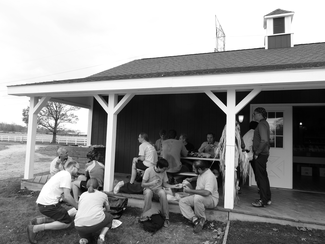
\includegraphics{cider-and-doughnuts.png} 

Cider and Doughnut Tour 2010

\small{{\tt kula.tproa.net/photos/2010/20101024-cider-doughnut-tour/ }}
\end{center}


\newpage

\thispagestyle{empty}
\vspace*{14cm}
\begin{sideways}
\Large{Thomas L. Kula}
\end{sideways}
\begin{sideways}
\Large{PO Box 980461}
\end{sideways}
\begin{sideways}
\Large{Ypsilanti MI 48198}
\end{sideways}


\end{document}


